\begin{figure}[H]
	\centering
	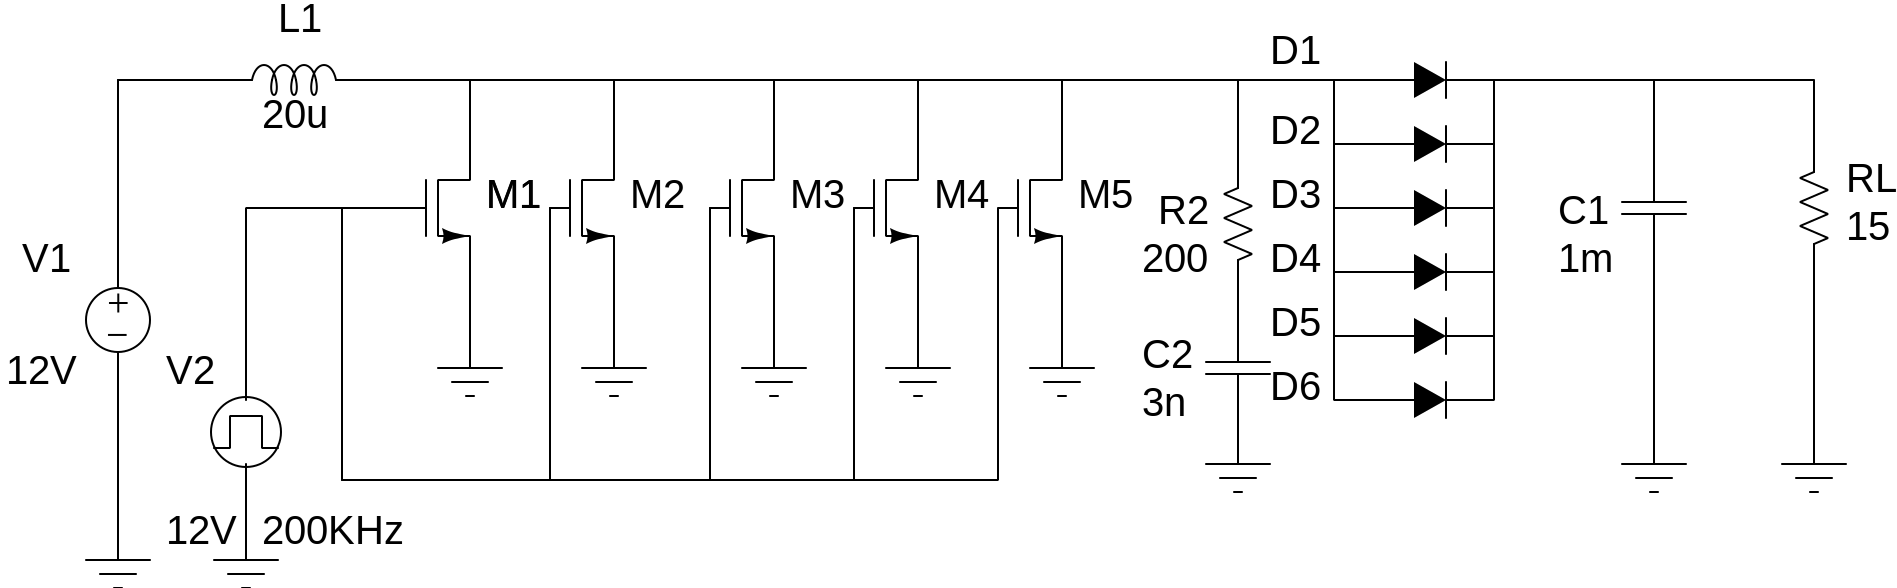
\includegraphics[scale=0.3]{Circ2}
	\caption{Circuito completo.}.
	\label{fig:Circ2}
\end{figure}

\Gus{Tiro ecuaciones que seguro se van a usar, al menos son las que use para intentar el calculo}


\begin{equation}
	{L} = \frac{(1-D) \cdot (V_s - V_E)}{2 \cdot f \cdot (I_{L_{max}} - I_{L_{prom}})}
\end{equation}

\Gus{verificar esta ecuacion}
\begin{equation}
	V_s = \frac{(V_E - V_{sat})}{1-D} - V_D \cdot (1 - D) 
	\label{ec:Nose}
\end{equation}

\Gus{Grafico XX de $I_S$ respecto al tiempo tengo que sacarlo de las diapos}

\begin{equation}
	I_s = \frac{I_{max} \cdot (1-D) \cdot T}{2 \cdot T} = \frac{I_{max} \cdot (1 - D)}{2} 
\end{equation}

Al estar trabajando en modo discontinuo se cumple que $ 2 I_{L_{prom}} =I_{L_{max}} $ por lo tanto.



\begin{equation}
	L = \frac{(1 - D)^2 \cdot (V_s - V_E)}{2 \cdot f \cdot (I_s)}
\end{equation}

Despejando y tomando a $\frac{V_s}{I_s} = R_L = \SI{15}{\ohm}$



\begin{equation}
	I_s^{-1} = \frac{\SI{15}{\ohm} - \frac{L \cdot 2 \cdot f}{(1-D)^2}}{V_E}
\end{equation}

\Gus{Aca se deberia seleccionar el D pero no se con que criterio, un criterio puede ser utilizando la otra ecuacion \eqref{ec:Nose} que da un valor similar en ambos casos}


Con $D=0,7$


\begin{equation}
	\boxed{I_s = \SI{1,963}{\ampere}}
\end{equation}


\begin{equation}
	\boxed{V_s = R_L \cdot I_s = \SI{29,45}{\volt}}
\end{equation}